\RequirePackage{luatex85}
\documentclass{article}
\usepackage{tikz, amsmath, mathtools}
\setlength\parindent{0mm}
\thispagestyle{empty}
\pagestyle{empty}

\usepackage{expl3}
\ExplSyntaxOn
\cs_new_eq:NN \Repeat \prg_replicate:nn
\ExplSyntaxOff
 
\usepackage[landscape, two column, margin=0.35in, column sep=0.7in]{geometry}

\everymath{\displaystyle}
\newcommand\stacktwo[2]{\(\begin{matrix}\text{#1}\\[-0.7ex]\text{#2}\end{matrix}\)}
\newcommand\stackthree[3]{\(\begin{matrix}\text{#1}\\[-0.7ex]\text{#2}\\[-0.7ex]\text{#3}\end{matrix}\)}
\newcommand\mylimit{{\lim_{\textstyle h\to\,\,\phantom{\text{\huge0}}}}}

\begin{document}
\Repeat{2}{
\section*{{\small 5 Minute Mini-Lesson} \\ The Limit Definition of Derivative}
\large
Suppose the height of a ball is a function of time $y=f(x)$.

\vspace{\stretch1}
\hfil
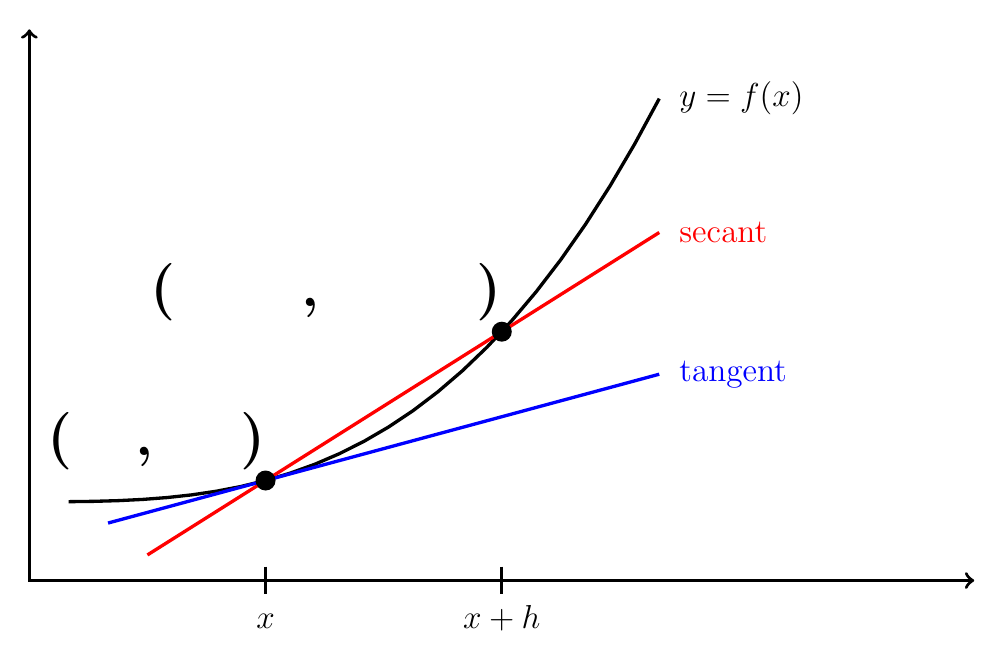
\begin{tikzpicture}[very thick]
% axes
\draw[<->] (0,7) to (0,0) to (12,0);
% f(x)
\draw[domain=0.5:8] plot (\x, \x^3/100+1) node [right] {\,\,\large$y=f(x)$};
% secant
\draw[red, domain=1.5:8] plot (\x, {3^3/100+1+(\x-3)*(6^3-3^3)/(6-3)/100})
node [right] {\,\,\large secant};
% tangent
\draw[blue, domain=1:8] plot (\x, {3^3/100+1+(\x-3)*3^2*3/100})
node [right] {\,\,\large tangent};
% closed circles
\foreach \x/\n in {3/x,6/x+h}{
\draw[black, fill=black] (\x, \x^3/100+1) circle (3pt) coordinate (\x);
\draw (\x, 5pt) -- ++(down:10pt) node[below] {\large$\n\vphantom h$};
}
\draw (3) node [above left] {\bfseries\huge(\hspace{8mm},\hspace{11mm})\!};
\draw (6) node [above left] {\bfseries\huge(\hspace{16mm},\hspace{20mm})\!};
\end{tikzpicture}

\vspace{\stretch2}
\(	\phantom\mylimit
	\scriptstyle
	\frac{\Delta y}{\Delta x}
	= \frac{y_2-y_1}{x_2-x_1}
	=
	\)

\bigskip
\(	 \phantom\mylimit
	\frac{\hspace{1in}}{}
	\)
= \stacktwo{slope of}{secant} 
= \stacktwo{difference}{quotient}
= \stackthree{average}{rate of}{change}
= \stacktwo{average}{velocity}

\vspace{\stretch2}
\(	 \mylimit
	\frac{\hspace{1in}}{}
	\)
= \stacktwo{slope of}{tangent} 
= derivative
= \stacktwo{rate of}{change}
= velocity

\vspace{\stretch3}
}
\end{document}
